\documentclass[conference]{IEEEtran}
\IEEEoverridecommandlockouts
% The preceding line is only needed to identify funding in the first footnote. If that is unneeded, please comment it out.
\usepackage{cite}
\usepackage{amsmath,amssymb,amsfonts}
\usepackage{algorithmic}
\usepackage{graphicx}
\usepackage{textcomp}
\usepackage{xcolor}
\usepackage[utf8]{inputenc}
\def\BibTeX{{\rm B\kern-.05em{\sc i\kern-.025em b}\kern-.08em
    T\kern-.1667em\lower.7ex\hbox{E}\kern-.125emX}}
\begin{document}

\title{A Deep Learning Approach for Higgs Boson Machine Learning Challenge\\
%{\footnotesize \textsuperscript{*}Note: Sub-titles are not captured in Xplore and
%should not be used}
%\thanks{Identify applicable funding agency here. If none, delete this.}
}

\author{\IEEEauthorblockN{Enrique Burga Gutiérrez}
\IEEEauthorblockA{\textit{Universidad Peruana de Ciencias Aplicadas} \\
Lima, Peru \\
u201411972@upc.edu.pe}
\and
\IEEEauthorblockN{Edwin Alfaro Paredes}
\IEEEauthorblockA{\textit{Universidad Peruana de Ciencias Aplicadas} \\
Lima, Peru \\
u201611810@upc.edu.pe}
}


\maketitle

\begin{abstract}
The objective of this paper is to find a deep learning method to classify new instances into "tau tau decay of a Higgs boson" or "background". To achieve the goal, we first made an analisys of the data to understand it. Then, we made cleaning tasks like impute the values with -999.0 and remove the irrelevant attributes. Finally, we tested different neuronal networks architecture to have a better result. We trained a deep neural network model and a convolutional network model. In both cases we obtained an accuracy of 82\% approximately.
\end{abstract}

\begin{IEEEkeywords}
Higgs, Boson, Deep Learning, Neural Networks, Physics
\end{IEEEkeywords}

\section{Introduction}
The Higgs Boson was announced in 2013 and its discovery was awarded with a Nobel Prize. The Higgs Boson is an elementary particle in the Standard Model of particle physics, produced by the quantum excitation of the Higgs field, one of the fields in particle physics theory \cite{b1}.
We extract the data from "The Higgs Challenge" in Kaggle\cite{b2}.\newline
We used Python in this work and the libraries were pandas, seaborn, scikit-learn and keras.\newline
To achieve the classification, first, we had to understand the data showing graphics, shape, and correlations between the attributes and the label. Then, we had to impute some attributes, because there were values that couldn't be computed by the ATLAS experiment and it is represented by the value "-999.0", also we remove some irrelevant attributes because they didn't correlate much with the label and we scale the attributes because we found outliers on it based on the box plot. Finally, we tested different neural network architecture to improve our results.
\section{Background}
\begin{itemize}
\item Neural Networks: They are models based on the human brain that are designed to recognize patterns in the data. They can help to cluster and classify \cite{b3}. Neural networks finds correlations and can learn to approximate an unknown function \begin{equation}f(x)=y\end{equation} where x is the input in the network and y is the output. The neural networks are composed by layers and each layer is made of nodes. The nodes combine the input from the data and the weights to amplify the input. These input-weight product are summed and passed to the activation function, which determines if it should pass through the network and its range limit to affect the final result.\newline
\item  Imputation of values: In this work we take the values with number "-999.0" as missing values, so we have to imputate them. Imputation is a process of replace missing data with substituted values to have a better prediction. To deal with missing values, there are different methods like remove the instance that contains it, infer the values using linear regression or replace the values with the mean of its attribute. In this case we use the imputation by mean because it give us a good correlation of each attribute with the label.
\end{itemize}


\section{Main Part}
In this section, we will describe step by step our way to have the final model. Starting with loading the dataset obtained from the website of the challenge, Kaggle\cite{b2}. Then, we will follow with the data exploration, where we will have to watch for attributes with outliers and the distribution of others. Next, preprocessing techniques will take part here. And finally, we will show the models of neural networks we have created to get a good accuracy.
\begin{figure}[htbp]
\centerline{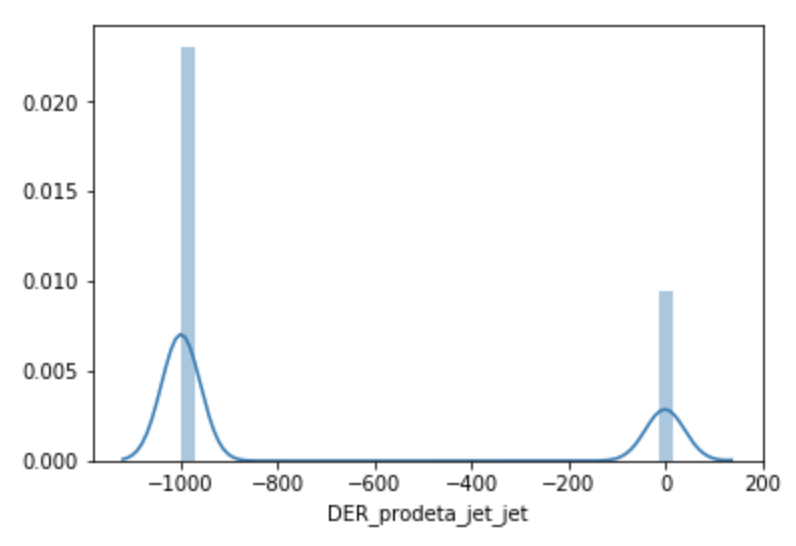
\includegraphics[width=\linewidth]{img1.png}}
\caption{Data distribution of \textit{DER Prodeta Jet Jet}.}
\label{fig}
\end{figure}
\begin{figure}[htbp]
\centerline{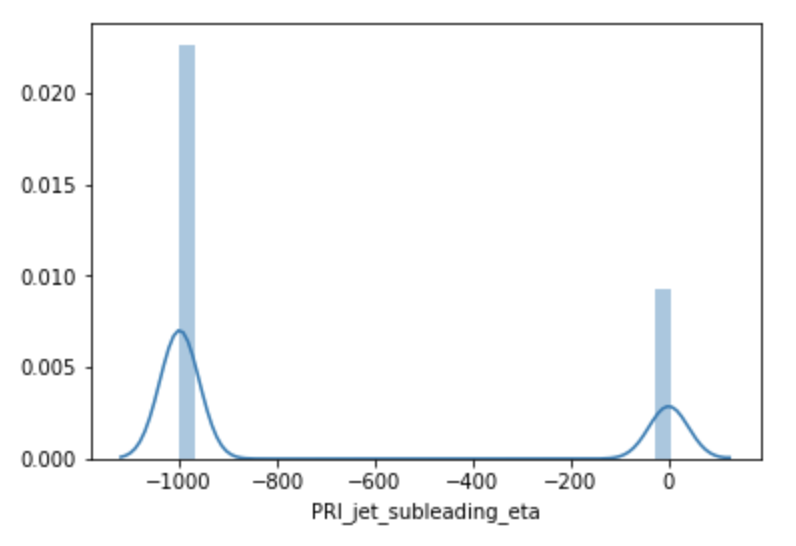
\includegraphics[width=\linewidth]{img2.png}}
\caption{Data distribution of \textit{PRI jet subleading eta}.}
\label{fig}
\end{figure}
\begin{figure}[htbp]
\centerline{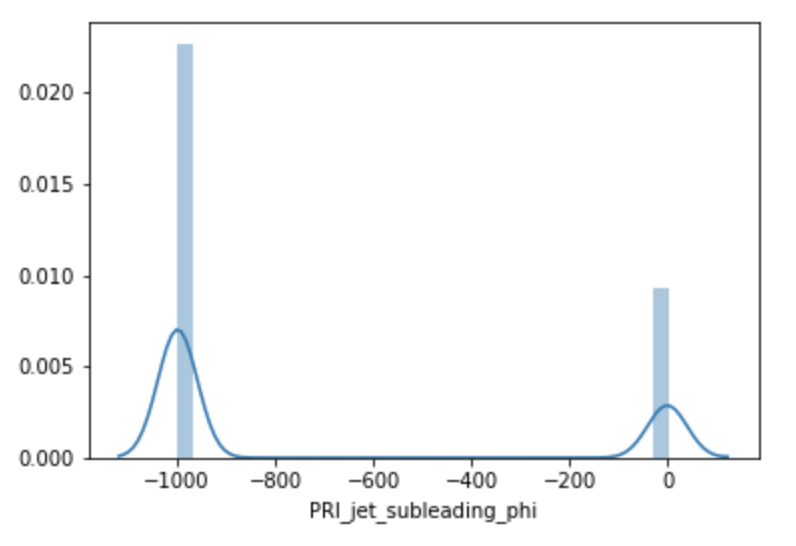
\includegraphics[width=\linewidth]{img3.png}}
\caption{Data distribution of \textit{PRI jet subleading phi}.}
\label{fig}
\end{figure}
\subsection{Exploratory Data Analysis and Preprocessing}\label{AA}
At the first part of the EDA, we will have to figure out how dispersed are the attributes of the dataset, and this will be show in Table I, we observed that just a few paremeters have a low standard deviation. Next, we found that there were many values -999 in a few of attributes. We can see this in the Fig. 1, Fig. 2 and Fig. 3. Also, we found an attribute called 'EventID', that is a counter from 1000 to 2500000 of our dataset, for this purpose the commented attribute will be removed.

How was mentioned earlier in this part, there were many values with the number -999, and based on the paper ofAdam-Bourdarios, et al.\cite{b1}. We noticed that this value means that the current instance does not have get that metric correctly. For this, we will removed the attributes that will have more than 30\% of the values like -999. The first attributes to remove are \textit{DER deltaeta jet jet}, \textit{DER mass jet jet}, \textit{DER prodeta jet jet}, \textit{DER lep eta centrality}, \textit{PRI jet leading pt}, \textit{PRI jet leading eta}, \textit{PRI jet leading phi}, \textit{PRI jet subleading pt}, \textit{PRI jet subleading eta} and \textit{PRI jet subleading phi}.

Thus, we have removed the attributes with more than 30\% with -999 values, but it remains one more that have -999 values but less than 30\%, and this is DER mass MMC. We replace the empty values by the mean of the rest of the values with no -999.

Next in our preprocessing, we will observe that there are a few parameters with a good pearson correlation coefficient with the attribute \textit{Label}, showed in the Table II. Besides, we plot a box graph for our remain attribute, how we can see in Fig. 4, Fig. 5 and Fig. 6, we observed that there are many outliers. So for that, we decided to apply a standard scaler by each instance in our dataset to get better results in our model predictor.

\begin{table}[h!]
  \begin{center}
    \caption{Higgs Boson Attributes Description}
    \label{tab:table1}
    \begin{tabular}{l|S|r}
      \textbf{Name} & \textbf{Mean} & \textbf{Std. Dev.}\\
      %$\alpha$ & $\beta$ & $\gamma$ \\
      \hline
      DER Mass MMC & -49.023079 & 406.345647\\
      DER Mass Transverse Met Lep & 49.239819 & 35.344886\\
      DER Mass Vis & 81.181982 & 40.828691\\ 
      DER Pt H & 57.895962 & 63.655682\\ 
      DER Deltaeta Jet Jet & -708.420675 & 454.480565\\ 
      DER Mass Jet Jet & -601.237051 & 657.972302\\ 
      DER Prodeta Jet Jet & -709.356603 & 453.019877\\ 
      DER Deltar Tau Lep & 2.373100 & 0.782911\\ 
      DER Pt Tot & 18.917332 & 22.273494\\ 
      DER Sum Pt & 158.432217 & 115.706115\\ 
      DER Pt Ratio Lep Tau & 1.437609 & 0.844743\\ 
      DER Met Phi Centrality & -0.128305 & 1.193585\\ 
      DER Lep Eta Centrality & -708.985189 & 453.596721\\ 
      PRI Tau Pt & 38.707419 & 22.412081\\
      PRI Tau Eta & -0.010973 & 1.214079\\
      PRI Tau Phi & -0.008171 & 1.816763\\
      PRI Lep Pt & 46.660207 & 22.064922\\
      PRI Lep Eta & -0.019507 & 1.264982\\
      PRI Lep Phi & 0.043543 & 1.816611\\
      PRI Met & 41.717235 & 32.894693\\
      PRI Met Phi & -0.010119 & 1.812223\\
      PRI Met Sumet & 209.797178 & 126.499506\\
      PRI Jet Num & 0.979176 & 0.977426\\
      PRI Jet Leading Pt & -348.329567 & 532.962789\\
      PRI Jet Leading Eta & -399.254314 & 489.338286\\
      PRI Jet Leading Phi & -399.259788 & 489.333883\\
      PRI Jet Subleading Pt & -692.381204 & 479.875496\\
      PRI Jet Subleading Eta & -709.121609 & 453.384624\\
      PRI Jet Subleading Phi & -709.118631 & 453.389017\\
      PRI Jet All Pt & 73.064591 & 98.015662\\
      Weight & 1.646767 & 1.875103\\
    \end{tabular}
  \end{center}
\end{table}

\begin{table}[h!]
  \begin{center}
    \caption{Pearson Metric Correlation with Label Attribute}
    \label{tab:table1}
    \begin{tabular}{l|S}
      \textbf{Name} & \textbf{Pearon Metric Correlation}\\
      %$\alpha$ & $\beta$ & $\gamma$ \\
      \hline
      DER Mass MMC & -0.010993564128142858\\
      DER Mass Transverse Met Lep & 0.35142795586167536\\
      DER Mass Vis & 0.014055273784852532\\ 
      DER Pt H & -0.19252632856874774\\ 
      DER Deltar Tau Lep & -0.012245481285482957\\ 
      DER Pt Tot & 0.015287426687781451\\ 
      DER Sum Pt & -0.15323593247581319\\ 
      DER Pt Ratio Lep Tau & 0.19539789618287828\\ 
      DER Met Phi Centrality & -0.27175187705164877\\ 
      PRI Tau Pt & -0.23523797587836734\\
      PRI Tau Eta & 0.0009432510582117519\\
      PRI Tau Phi & 0.004402538686388409\\
      PRI Lep Pt & 0.03194758680534819\\
      PRI Lep Eta & -0.0015162353770597238\\
      PRI Lep Phi & -0.004125447411524848\\
      PRI Met & -0.022465751510785878\\
      PRI Met Phi & -0.007475342188590254\\
      PRI Met Sumet & -0.13552026152268465\\
      PRI Jet Num & -0.1335491230816916\\
      PRI Jet All Pt & -0.13429572666925305\\
      Weight & 0.6309817159733314\\
    \end{tabular}
  \end{center}
\end{table}


\begin{figure}[htbp]
\centerline{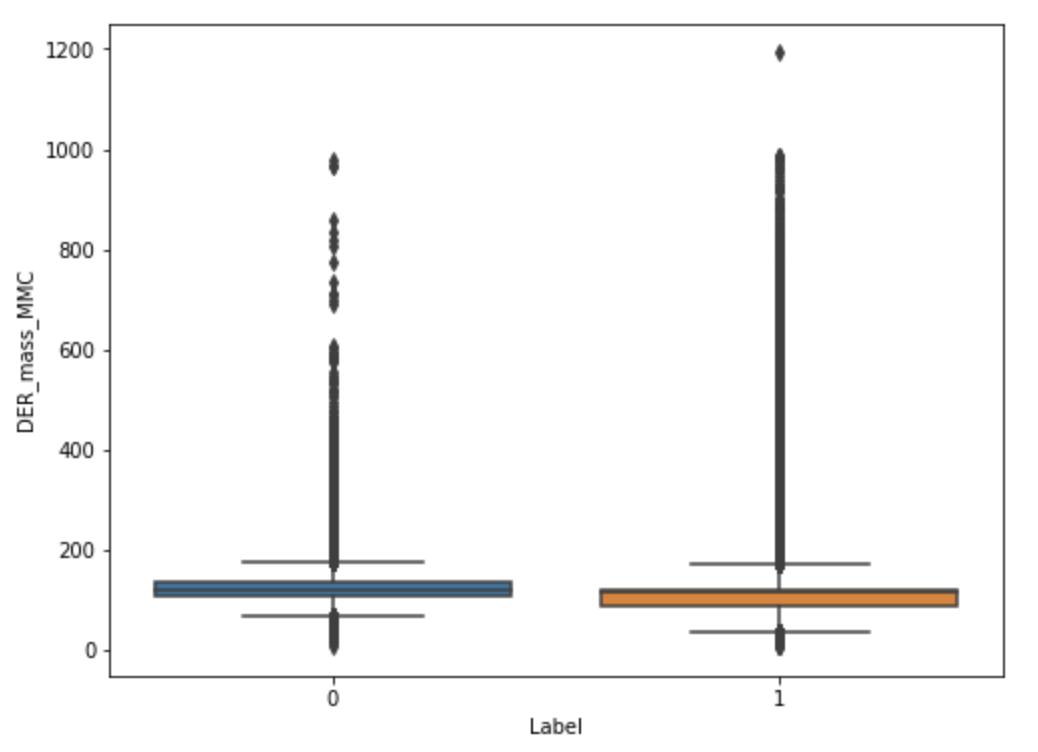
\includegraphics[width=\linewidth]{img4.png}}
\caption{Data Distribution of \textit{Box Plot of attribute \textit{DER Mass MMC} by \textit{Label}}.}
\label{fig}
\end{figure}


\begin{figure}[htbp]
\centerline{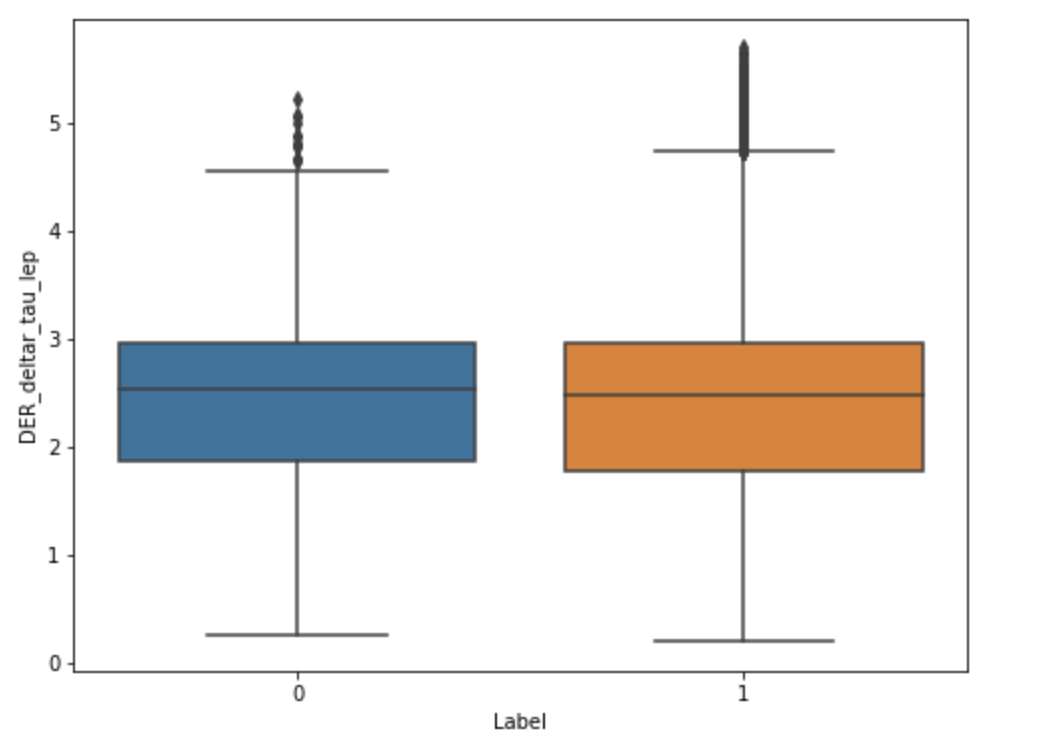
\includegraphics[width=\linewidth]{img5.png}}
\caption{Data Distribution of \textit{Box Plot of attribute \textit{DER Deltar Tau Lep} by \textit{Label}}.}
\label{fig}
\end{figure}

\begin{figure}[htbp]
\centerline{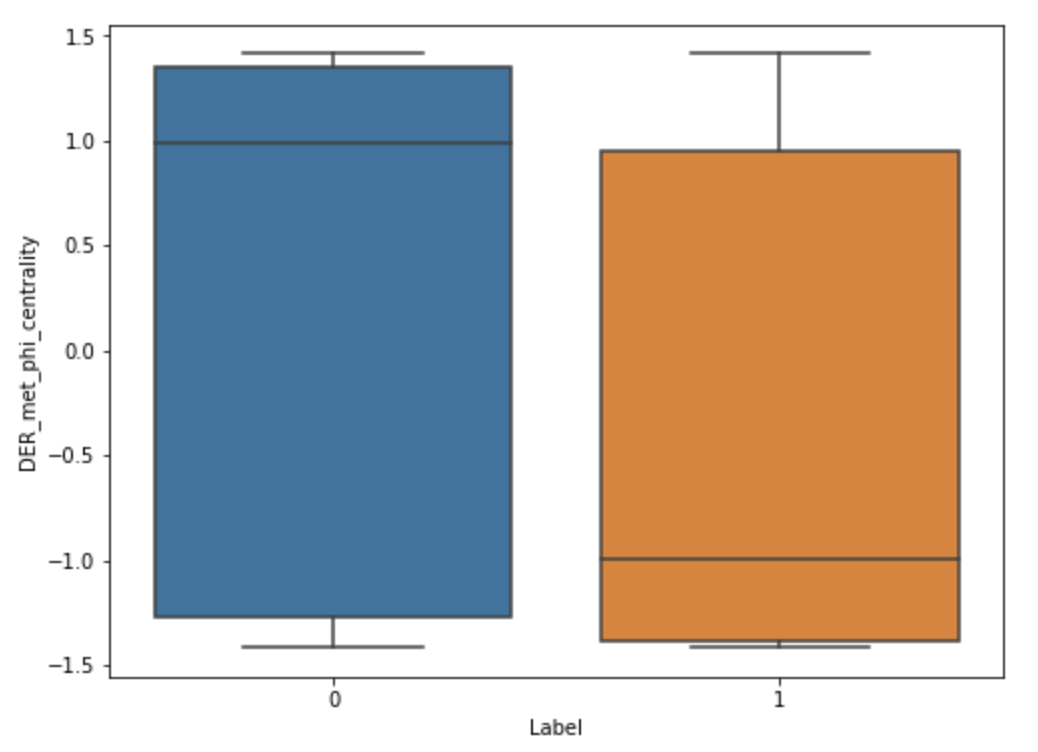
\includegraphics[width=\linewidth]{img6.png}}
\caption{Data Distribution of \textit{Box Plot of attribute \textit{DER Met Phi Centrality} by \textit{Label}}.}
\label{fig}
\end{figure}
	 

\subsection{Model}\label{AA}
For the model, we have worked with two approaches. The first one is the application of a Classic Deep Neural Network, using bach size of 4000 and 30 epochs. Here we implement a deep neural network with 2 hidden layers, 1 input layer and 1 output layer. Each layer will have the application of a dropout layer by random purposes. Hidden layers will have the relu activation function and sigmoid activation for the output layer.

The next approach was the application of a One Dimension Convolutional Neural Network, with the layers of Convolution, 2 layers of Pooling, 1 layers of faltten and 4 layers of dense. For the two models, we use the adam optimizer, and the loss binary cross entropy.


\subsection{Results}\label{AA}
For our two approches, we get an accuracy of around 82.0\% of accuracy and 40.0\% of loss, how we can see in the Fig. 7 and Fig. 8. Also, our result has a ROC AUC value of 79.86\%.


\begin{figure}[htbp]
\centerline{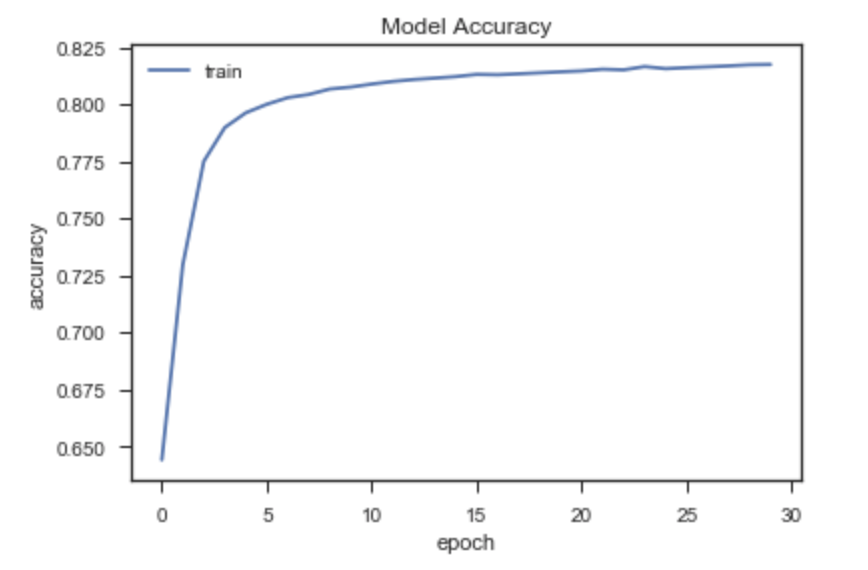
\includegraphics[width=\linewidth]{img7.png}}
\caption{Accuracy vs Epochs.}
\label{fig}
\end{figure}


\begin{figure}[htbp]
\centerline{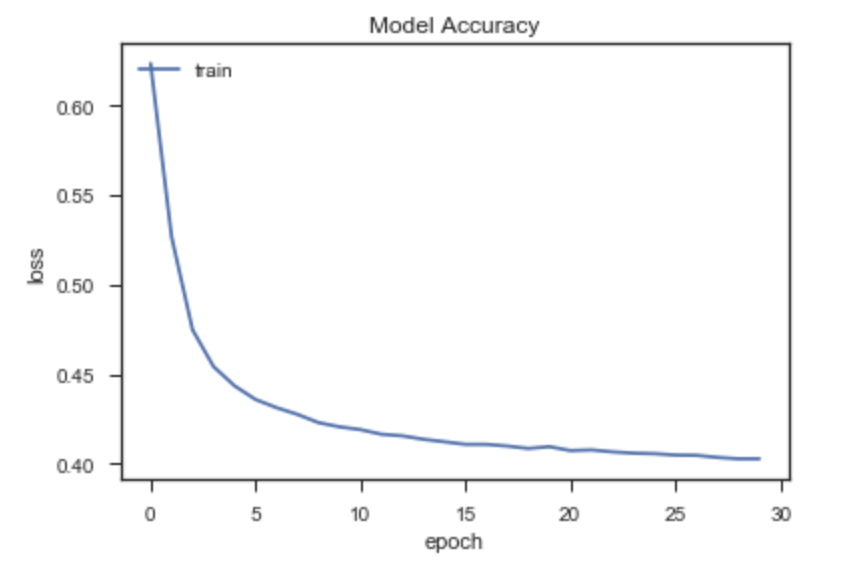
\includegraphics[width=\linewidth]{img8.png}}
\caption{Loss vs Epochs.}
\label{fig}
\end{figure}

\section{Related works}
\begin{itemize}
\item Machine learning techniques in searches for tth in the h → bb decay channel: In this paper the authors try to detect tth in the h → bb decay channel. The authors tested 8 different machine learning methods, but 2 of them outperform the others. They were extreme gradient boosted trees and neural network models \cite{b4}.\newline
\item Searching for Exotic Particles in High-Energy Physics with Deep Learning: The objective of this paper is find rare particles solving difficult signal-versus-background classification problems. The authors demonstrate that deep learning methods need no manually constructed inputs and yet improve the classification metric by as much as 8\% over the best current approaches \cite{b5}.\newline
\item  ML2014: Higgs Boson Machine Learning Challenge: In this paper, the authors solve the Higgs Boson Machine Learning Challenge \cite{b6}.\newline
\item Learning to discover: the Higgs Boson Machine Learning Challenge: In this paper, the authors explain all the process including analysis, preprocessing and construction of the model to solve the Higgs Boson Machine Learning Challenge \cite{b1}.
\end{itemize} 

\section{Conclusions and Future Work}
After a while experimenting with many parameters inside our two approches, we found that both achieved an accuracy of 82\%. It is necessary to experiment with other architectures inside a Classic Deep Neural Network and in the Convolutional Neural Network. Although is possible to say that we can use other types of neural networks, as a Recurrent Neural Network or a Generative Neural Network.


\begin{thebibliography}{00}
\bibitem{b1} C. Adam-Bourdarios, G. Cowan, C. Germain, I.Guyon, B. Kégl, and D. Rousseau, ``Learning to discover: the Higgs boson machine learning challenge'', July 2014
\bibitem{b2} Kaggle, https://www.kaggle.com/c/higgs-boson/overview, May 2014
\bibitem{b3} Skymind, https://skymind.ai/wiki/neural-network
\bibitem{b4} R. Santos, M. Nguyen, J. Adelman, and J. Zhou, ``Machine learning techniques in searches for tth in the h → bb decay channel'', November 2016.
\bibitem{b5} P. Baldi, P. Sadowski, and D. Whiteson, ``Searching for Exotic Particles in High-Energy Physics with Deep Learning'', June 2014
\bibitem{b6} J. Perez, R. Ponmalai, A. Silver, and D. Strack, ``ML2014: Higgs Boson Machine Learning Challenge'', August 2014
\end{thebibliography}
\vspace{12pt}
\color{red}
\end{document}
